\documentclass[10pt,a4paper]{article}

\usepackage[utf8]{inputenc}
\usepackage[T1]{fontenc}
\usepackage[italian]{babel}
\usepackage{graphicx}
\usepackage{amsmath,amssymb,amsfonts}
\usepackage{caption}
\usepackage{subcaption}
\usepackage{wrapfig}
\usepackage{float}
\usepackage{geometry}
\geometry{top=2.5cm, bottom=2.5cm, left=1.7cm, right=1.7cm}
\usepackage{fancyhdr}
\usepackage{titlesec}
\usepackage{lmodern}
\usepackage{caption}
\usepackage{comment}
\usepackage{booktabs}
\usepackage{makecell}
\usepackage{siunitx}
\usepackage[version=4]{mhchem} 
\DeclareCaptionFont{myit}{\footnotesize\itshape\fontfamily{cmr}\selectfont}
\captionsetup{
    font=myit,
    labelfont={bf},
    textfont=normalfont
}
\usepackage{titletoc}

% Intestazioni moderne
\pagestyle{fancy}
\fancyhf{}
\fancyhead[L]{Vita media del $\mu$}
\fancyhead[R]{Niccolò Menichetti \\ Luca Musetti \\ Luca Nasone}
\fancyfoot[C]{\thepage}

% Re e Im
\renewcommand{\Re}{\mathop{\mathrm{Re}}}
\renewcommand{\Im}{\mathop{\mathrm{Im}}}

% Per "simulare" capitoli
\newcommand{\chapter}[1]{
    \clearpage
    \section*{#1}
    \addcontentsline{toc}{section}{#1}
}

\title{\bfseries Relazione di laboratorio \\[1ex] \Large Vita media del $\mu$}
\author{Niccolò Menichetti \\ Luca Musetti \\ Luca Nasone}
\date{Anno Accademico 2025--2026}

\begin{document}

\begin{titlepage}
    \thispagestyle{empty}
    
    \begin{figure}[ht]
        \centering
        \begin{minipage}{0.48\textwidth}
            \centering
            
\includegraphics[width=5.0cm]{Stemma_unipi.svg.png}
        \end{minipage}%
        \hfill
        \begin{minipage}{0.48\textwidth}
            \centering
            
\includegraphics[width=7.0cm]{unipi_fermi.png}
        \end{minipage}
    \end{figure}

    \vspace{4.0cm} % Spazio per centrare verticalmente il contenuto

    \begin{center}
        {\fontsize{20pt}{24pt}\selectfont\bfseries Vita media del muone}\\[0.3cm]
        {\large Relazione laboratorio di interazioni fondamentali}\\[9.0cm]

        {\Large NICCOLO' MENICHETTI\hspace{0.2cm} LUCA MUSETTI \hspace{0.2cm} LUCA NASONE}\\[0.35cm]
        {\normalsize Anno Accademico 2025 - 2026}
    \end{center}

\end{titlepage}

\newpage

\begin{abstract}
        
    \emph{Nella seguente relazione descriviamo la nostra misura della vita media del muone, effettuata sui muoni dei raggi cosmici. Otteniamo una vita media pari a ...(To be continued...)}
        
\end{abstract}

\tableofcontents

\newpage

\section{Introduzione}

Sappiamo che, a causa dell'interazione con l'atmosfera, i raggi cosmici che arrivano dallo spazio hanno una composizione differente a livello del mare. In particolare prevalgono i muoni $\mu$, che decadono nel seguente modo:

\begin{center}
    \ce{$\mu^{-}\rightarrow e^{-}\bar \nu_e \nu_{\mu}$}
\end{center}

con vita media è $\tau_{\mu} = 2.1969811 \pm 0.0000022 $ $\mu s$ (PDG 2025) e carica $\pm e$.

L'obiettivo dell'esperimento è misurare il valore della vita media del muone, con un apparato sperimentale in grado di rilevare i raggi cosmici e fermare i $\mu$ a bassa energia. 

Nella materia i muoni negativi tendono a formare degli stati legati con i nuclei (atomi mesici). Questo fatto rende la vita media del muone con carica negativa più bassa di quella per muoni con carica positiva. Con i dati a nostra disposizione possiamo estrarre l'abbondanza relativa di una specie rispetto all'altra, ossia $N_+/N_-$, note le popolazioni $N_+$ e $N_-$ per i muoni con la carica $\pm e$ rispettivamente.

Utilizzando gli impulsi rilasciati nei fotomoltiplicatori, è stato possibile, previa un'opportuna calibrazione, misurare lo spettro in energia dell'$e^{-}$ prodotto dal decadimento. Essendo un decadimento a 3 corpi, sappiamo che per certo non è monocromatico, ma si ricava facilmente dalla cinematica relativistica che è limitato superiormente da:

\begin{center}
    $(E_e)^{max} = \frac{m_{\mu}^2+m_{e}^2}{2m_{\mu}}$
\end{center}

da quest'ultima misura sarà possibile ottenere una stima della massa del $\mu$, osservando il valore di energia dove osservo una discesa.

\section{Apparato sperimentale}

\begin{figure}[h]
\centering
\begin{minipage}{0.40\textwidth}
    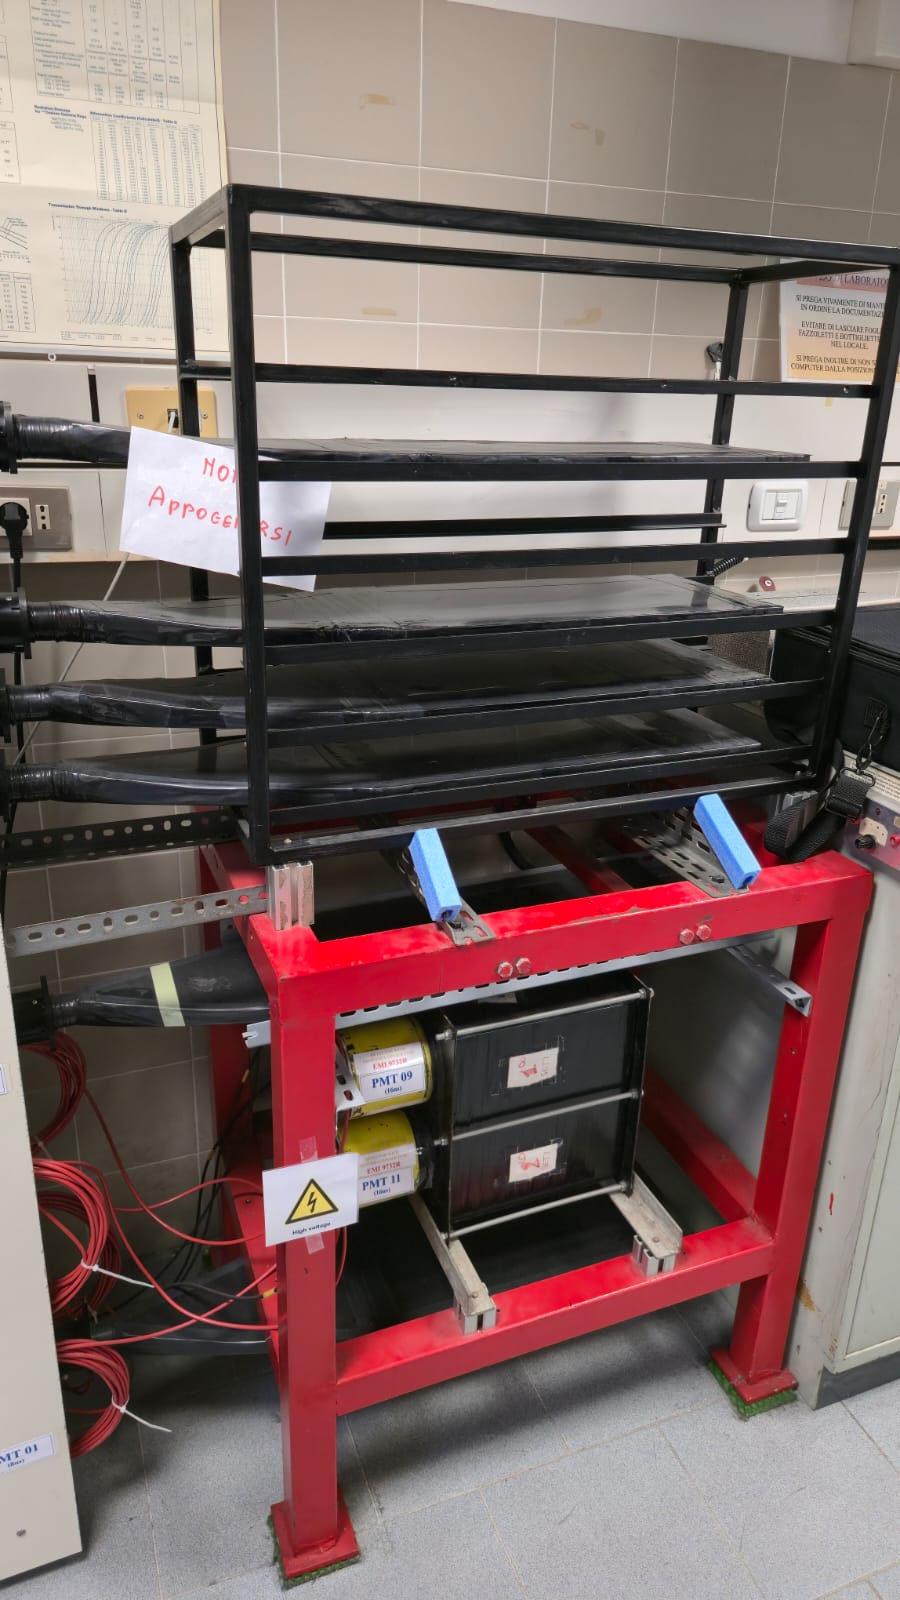
\includegraphics[width=0.55\textwidth]{WhatsApp Image 2025-12-06 at 15.04.09 (3).jpeg}
    \caption{Sistema Telescopio+Blocco+VETO}
\end{minipage}
\begin{minipage}{0.4\textwidth}
    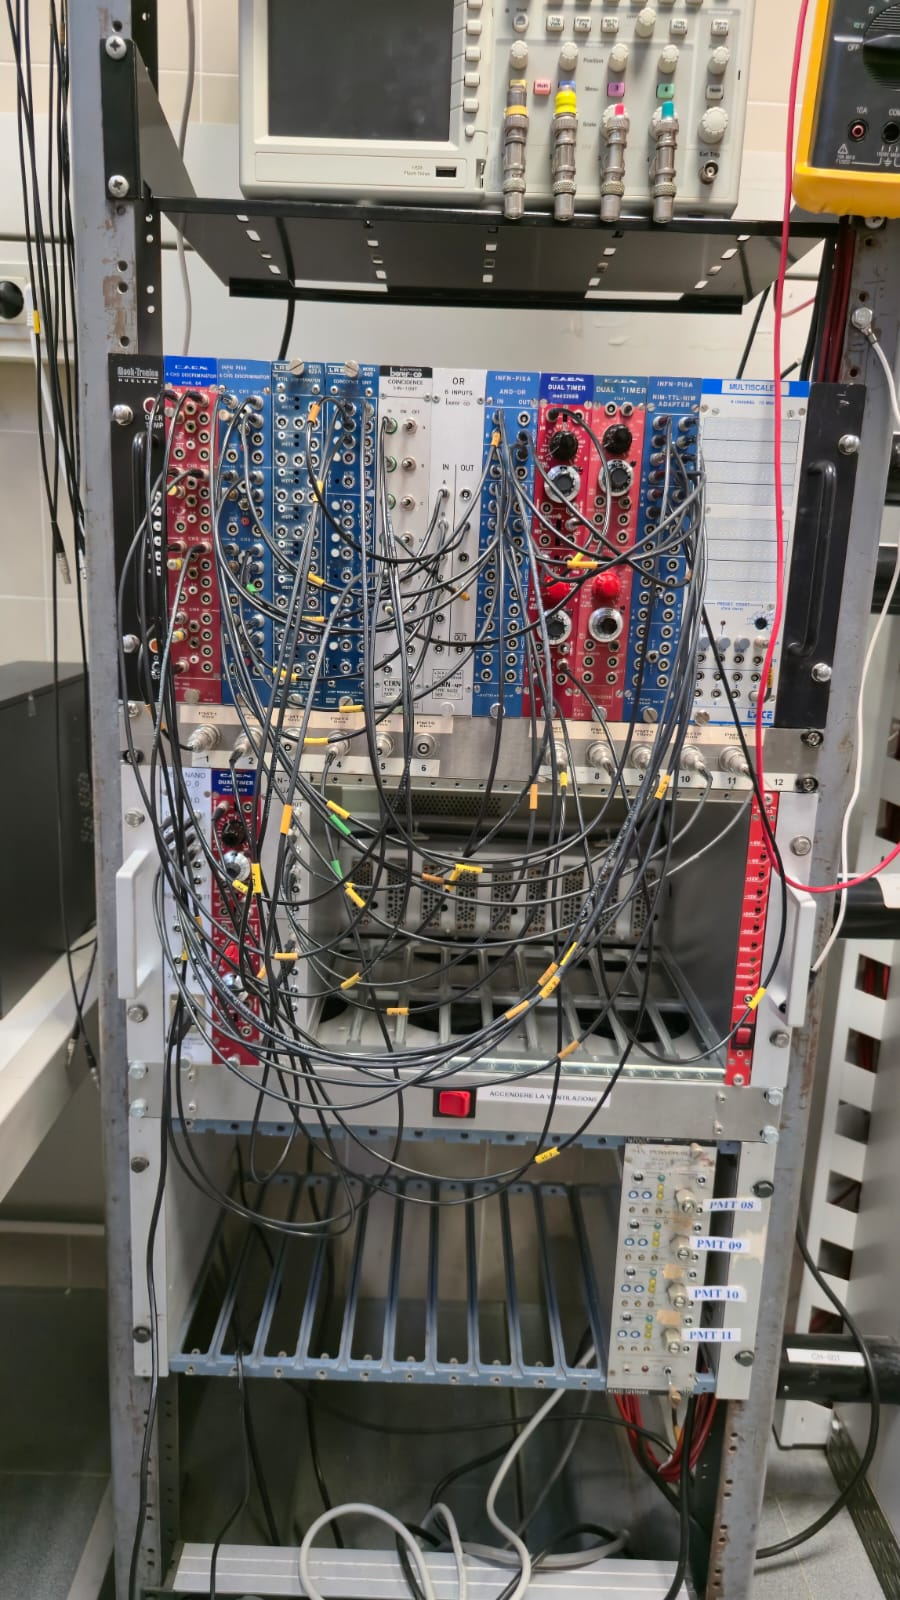
\includegraphics[width=0.55\textwidth]{WhatsApp Image 2025-12-06 at 15.04.09 (2).jpeg}
    \caption{Apparato di lettura dei segnali ricevuti dai PMT}
\end{minipage}
\end{figure}

\begin{itemize}
\item 6 lastre di scintillatore lette ciascuno da un fotomoltiplicatore (PMT), dimensioni (49.8 $\pm$ 0.1 cm) $\times$ (27.5 $\pm$ 0.1 cm) $\times$ (2.3 $\pm$ 0.1 cm);
\item 1 blocco di scintillatore letto da 4 PMT, dimensioni (30.0 $\pm$ 0.1 cm) $\times$ (31.0 $\pm$ 0.1 cm) $\times$ (31.0 $\pm$ 0.1) ;
\item una scheda DE0-10 NANO;
\item 2 discriminatori (NIM CAEN N84 e NIM INFN);
\item 3 unità di coincidenza (NIM LRS 465, NIM CERN N6234, NIM);
\item 1 unità di OR (NIM CERN);
\item 2 unità di Dual Timer (NIM CAEN mod2255B e NIM CAEN N2255);
\item 1 unità di conversione NIM-TTL;
\item 1 multiscaler (NIM INFN Multiscaler130);
\item 1 unità di Fan-Out;
\item 1 integratore analogico (NIM CAEN N914);
\item 1 ADC (NIM CAEN N6725);
\item 1 oscilloscopio;
\item 2 computer, per regolare le alimentazioni e per le acquisizioni;
\item 1 multimetro;
\item cavi coassiali di vario ritardo e terminazioni a 50 e 0 $\Omega$;
\item 1 metro a nastro;
\end{itemize}

\newpage

\section{Punto di lavoro}

\subsection{Telescopio}

La prima attività svolta in laboratorio è stato scegliere il punto di lavoro dei vari PMT. Soglie e alimentazioni influenzano l'efficienza e di conseguenza il numero di eventi rivelati. Vogliamo sia più alta possibile in modo da massimizzare la statistica a nostra disposizione. 

Sono stati scelti il PMT07, il PMT04 e il PMT02. Come stima dell'efficienza di un PMT (poniamo ad esempio il PMT07) abbiamo usato il rapporto fra le coincidenze triple $(07\land04\land02)$ e le coincidenze doppie degli altri due (nel nostro esempio $(04\&02)$). 

Misuriamo i conteggi combinando i segnali discriminati tramite le unità di coincidenza, le cui uscite sono in seguito inviate al multiscaler, che conta per 100 s. La misura viene poi ripetuta variando l'alimentazione.

Durante la procedura sono state misurate anche le singole dei due PMT usati per le coincidenze doppie, in quanto il loro rate in singola influenza il rate delle doppie false, ottenuto da:

\begin{center}

    $ R_{fake} = R_1 R_2 (w_1 + w_2 - 2w)$

\end{center}

Dove $R_1$ e $R_2$ sono i rate in singola dei PMT di interesse, $w_1$ e $w_2$ sono le durate dei loro segnali discriminati (50 ns nel nostro caso). $w$ è la sovrapposizione temporale minima per avere una coincidenza, di 2 ns. Sceglieremo alimentazioni e soglie cercando di rendere il numero di doppie false trascurabile rispetto alle doppie misurate.

Tale procedura è ottimale per il PMT mediano (il PMT04), ma non per il PMT07 e PMT02, a causa della geometria del sistema. 
Per correggere tale effetto abbiamo simulato il sistema con un Montecarlo in modo da ricavare la probabilità che un raggio cosmico passi per un PMT dato il passaggio dagli altri due (accettanza). Dividendo il rapporto triple su doppie con tale valore si ottiene una stima più accurata dell'efficienza.

Stimiamo l'errore sul rapporto triple su doppie con: 

\begin{center}

    $ \sigma_{\varepsilon} = \sqrt{\frac{\varepsilon(1-\varepsilon)}{D}}$
  
\end{center}

$D$ è il numero di doppie.

Riportiamo di seguito le curve di efficienza : 

\begin{figure}[h]
\centering

\includegraphics[width = 0.7\textwidth]{Efficiency Curves - Telescope.png}
\caption{Grafico delle curve di efficenza per i PMT02, -04, -07}
\end{figure}

Riportiamo le misure fatte nelle tabelle sottostanti, le colonne sono voltaggio di alimentazione, efficienza, errore sull'efficienza e numero di doppie fake, con il titolo che si riferisce al PMT per cui si sono eseguite le misure:

\newpage

\begin{center}

\begin{minipage}{0.32\textwidth}
\centering
\textbf{PMT02}

\vspace{0.25cm}

\begin{tabular}{|c|c|c|c|}
\toprule
$HV$[kV]& $\varepsilon$ [$\%$] & $\sigma_{\varepsilon}$[$\%$] & $D_{fake}$ \\
\midrule
1.675 & 52 & $\pm$ 2 & 0.69 \\
1.700 & 70 & $\pm$ 2 & 0.65 \\
1.720 & 80 & $\pm$ 1 & 0.63 \\
1.730 & 81 & $\pm$ 1 & 0.59 \\
1.750 & 89 & $\pm$ 1 & 0.53 \\
1.775 & 80 & $\pm$ 1 & 0.54 \\
1.800 & 91 & $\pm$ 1 & 0.56 \\
\bottomrule
\end{tabular}
\end{minipage}
\hfill
\begin{minipage}{0.32\textwidth}
\centering
\textbf{PMT04}

\vspace{0.25cm}

\begin{tabular}{|c|c|c|c|}
\toprule
$HV$[kV]& $\varepsilon$ [$\%$] & $\sigma_{\varepsilon}$[$\%$] & $D_{fake}$ \\
\midrule
1.675 & 87 & $\pm$ 2 & 0.077 \\
1.700 & 94 & $\pm$ 1 & 0.068 \\
1.720 & 94 & $\pm$ 1 & 0.074 \\
1.730 & 92 & $\pm$ 2 & 0.073 \\
1.750 & 93 & $\pm$ 1 & 0.078 \\
1.775 & 94 & $\pm$ 1 & 0.076 \\
1.800 & 92 & $\pm$ 1 & 0.076 \\
\bottomrule
\end{tabular}
\end{minipage}
\hfill
\begin{minipage}{0.32\textwidth}
\centering
\textbf{PMT07}

\vspace{0.25cm}

\begin{tabular}{|c|c|c|c|}
\toprule
$HV$[kV]& $\varepsilon$ [$\%$] & $\sigma_{\varepsilon}$[$\%$] & $D_{fake}$ \\
\midrule
1.675 & 50 & $\pm$ 2 & 0.97 \\
1.700 & 77 & $\pm$ 2 & 0.79 \\
1.720 & 83 & $\pm$ 1 & 0.73 \\
1.730 & 78 & $\pm$ 2 & 0.73 \\
1.750 & 80 & $\pm$ 2 & 0.68 \\
1.775 & 92 & $\pm$ 1 & 0.64 \\
1.800 & 88 & $\pm$ 1 & 0.57 \\
\bottomrule
\end{tabular}
\end{minipage}

\vspace{1.2cm}

\textbf{In conclusione il punto di lavoro scelto per il telescopio è:}

\vspace{0.6cm}

\begin{tabular}{|c|c|c|c|}
\toprule
Parametro & PMT02 & PMT04 & PMT07 \\
\midrule
$V_{supply}$ [kV] & 1.750 & 1.700 & 1.750 \\
$V_{thr}$ [mV] & -30 & -30 & -30 \\
$\varepsilon$ [$\%$] & 88 & 94 & 79 \\
\bottomrule
\end{tabular}

\end{center}


\subsection{Bersaglio}

Abbiamo fatto uno studio analogo per il bersaglio, in questo caso, al fine di creare una geometria favorevole alla misura di efficienza, abbiamo variato gli scintillatori usati, riportiamo le combinazioni usate per ciascun PMT del blocco:

\begin{itemize}

\item PMT08 : PMT02-PMT08-PMT10 
\item PMT09 : PMT02-PMT09-PMT01
\item PMT10 : PMT07-PMT08-PMT10
\item PMT11 : PMT09-PMT11-PMT01

\end{itemize}

Per PMT08-09-11 si è usato il metodo dei trigger ortogonali con lo scintillatore immediatamente sopra/sotto.
Può sicuramente sembrare insolito il PMT10, la ragione è che esso è fuori asse col PMT01, quindi non ci è sembrato ragionevole usarlo. Invece usando il PMT08 (immediatamente sopra) e il PMT07 (il più in alto di tutti) abbiamo pensato potesse stringere opportunamente l'angolo solido, in modo da aumentare l'accettanza e dunque avere una stima più veritiera dell'efficienza partendo dal rapporto triple su doppie. 
Per il resto, le misure di rate si sono svolte come descritto nella sezione precedente, così come le stime di errore.

Riportiamo come sopra grafico e misure in tabella:

\begin{figure}[h]
    \centering
    
\includegraphics[width=0.5\linewidth]{Efficiency Curves - Target.png}
    \caption{Curve di efficienza per i PMT di lettura del bersaglio}
    \label{fig:placeholder}
\end{figure}

\newpage

\begin{center}

% ---------- PRIMA RIGA ----------
\begin{minipage}{0.48\textwidth}
\centering
\textbf{PMT08}

\vspace{0.25cm}

\begin{tabular}{|r|r|r|r|}
\toprule
HV [kV] & $\varepsilon [\%]$ & $\sigma_{\varepsilon} [\%]$ & $D_{fake}$ \\
\midrule
1.100 & 76 & $\pm$ 2 & 0.01 \\
1.130 & 81 & $\pm$ 2 & 0.02 \\
1.150 & 80 & $\pm$ 2 & 0.02 \\
1.175 & 74 & $\pm$ 2 & 0.03 \\
1.200 & 82 & $\pm$ 2 & 0.04 \\
1.230 & 82 & $\pm$ 2 & 0.06 \\
1.250 & 78 & $\pm$ 2 & 0.07 \\
\bottomrule
\end{tabular}
\end{minipage}
\hfill
\begin{minipage}{0.48\textwidth}
\centering
\textbf{PMT10}

\vspace{0.25cm}

\begin{tabular}{|r|r|r|r|}
\toprule
HV [kV] & $\varepsilon [\%]$ & $\sigma_{\varepsilon} [\%]$ & $D_{fake}$ \\
\midrule
1.070 & 53 & $\pm$ 5 & 0.054 \\
1.100 & 60 & $\pm$ 5 & 0.047 \\
1.150 & 64 & $\pm$ 4 & 0.055 \\
1.170 & 56 & $\pm$ 5 & 0.054 \\
1.200 & 56 & $\pm$ 5 & 0.059 \\
1.230 & 59 & $\pm$ 5 & 0.054 \\
\bottomrule
\end{tabular}
\end{minipage}

\vspace{1cm}

% ---------- SECONDA RIGA ----------
\begin{minipage}{0.48\textwidth}
\centering
\textbf{PMT09}

\vspace{0.25cm}

\begin{tabular}{|r|r|r|r|}
\toprule
HV [kV] & $\varepsilon [\%]$ & $\sigma_{\varepsilon} [\%]$ & $D_{fake}$ \\
\midrule
1.100 & 75 & $\pm$ 2 & 0.080 \\
1.130 & 76 & $\pm$ 2 & 0.076 \\
1.170 & 76 & $\pm$ 2 & 0.077 \\
1.200 & 81 & $\pm$ 2 & 0.077 \\
1.230 & 78 & $\pm$ 2 & 0.078 \\
1.250 & 77 & $\pm$ 2 & 0.079 \\
1.277 & 84 & $\pm$ 2 & 0.077 \\
1.300 & 86 & $\pm$ 2 & 0.079 \\
\bottomrule
\end{tabular}
\end{minipage}
\hfill
\begin{minipage}{0.48\textwidth}
\centering
\textbf{PMT11}

\vspace{0.25cm}

\begin{tabular}{|r|r|r|r|}
\toprule
HV [kV] & $\varepsilon [\%]$ & $\sigma_{\varepsilon} [\%]$ & $D_{fake}$ \\
\midrule
1.100 & 74 & $\pm$ 2 & 0.077 \\
1.130 & 76 & $\pm$ 2 & 0.077 \\
1.170 & 76 & $\pm$ 2 & 0.077 \\
1.200 & 81 & $\pm$ 2 & 0.077 \\
1.230 & 78 & $\pm$ 2 & 0.077 \\
1.250 & 79 & $\pm$ 2 & 0.079 \\
1.277 & 84 & $\pm$ 2 & 0.080 \\
1.300 & 86 & $\pm$ 2 & 0.079 \\
\bottomrule
\end{tabular}
\end{minipage}

\vspace{1.2cm}

\textbf{Il punto di lavoro scelto è stato dunque:}

\vspace{0.6cm}

\begin{tabular}{|r|r|r|r|r|}
\toprule
Parametro & PMT08 & PMT09 & PMT10 & PMT11 \\
\midrule
$V_{supply}$ [kV] & 1.26  & 1.32  & 1.26  & 1.26  \\
$V_{thr}$ [mV] & -80 & -80 & -80 & -80 \\
$\varepsilon$ [$\%$] & 78  & 85  & 58 & 87 \\
\bottomrule
\end{tabular}

\end{center}


\subsection{VETO}

Infine abbiamo eseguito lo studio analogo per il PMT di VETO, ossia il PMT01, quello immediatamente sotto il bersaglio. Abbiamo usato il rapporto triple su doppie della terna PMT07 - PMT09 $\vee$ PMT11 - PMT01. 
Il ragionamento per la scelta è analogo al caso precedente del PMT10, in questo caso il problema è la posizione dello scintillatore, per il quale non è presente una lastra sottostante.
Riportiamo sempre grafico e tabella: 


\begin{figure}[h]
\centering

\begin{minipage}{0.52\textwidth}
\centering

\includegraphics[width=\linewidth]{Efficiency Curves - VETO.png}
\caption{Curva di efficienza per il PMT scelto come VETO}
\label{fig:veto_efficiency}
\end{minipage}
\hfill
\begin{minipage}{0.42\textwidth}
\centering
\textbf{PMT01}

\vspace{0.25cm}

\begin{tabular}{|r|r|r|r|}
\toprule
HV [kV] & $\varepsilon [\%]$ & $\sigma_{\varepsilon} [\%]$ & $D_{fake}$ \\
\midrule
1.630 & 48 & $\pm$ 4 & 0.35 \\
1.650 & 56 & $\pm$ 4 & 0.35 \\
1.675 & 55 & $\pm$ 4 & 0.33 \\
1.700 & 55 & $\pm$ 4 & 0.34 \\
1.720 & 52 & $\pm$ 4 & 0.34 \\
1.730 & 56 & $\pm$ 4 & 0.33 \\
1.750 & 52 & $\pm$ 4 & 0.36 \\
\bottomrule
\end{tabular}
\end{minipage}

\end{figure}

\newpage

\section{Presa dati}

\subsection{Selezione degli eventi}

Per la misura di tempo, necessitiamo di due segnali, uno che ci dica quando il muone si è fermato (START) e uno che ci dica quando è decaduto (STOP). La differenza fra i tempi in cui ho registrato STOP e START, ci fornisce il tempo in cui il $\mu$ è decaduto.

In questa sezione trattiamo la caratterizzazione dei segnali di START e STOP. Essi sono ottenuti con opportune combinazioni logiche dei segnali in uscita dai PMT e digitalizzati dai discriminatori. Inoltre, abbiamo usato l'unità di timer, un modulo in grado di generare un segnale logico su un segnale di trigger a scelta. Ci riferiamo a tale segnale con $GATE$, e può essere modificato in base alle necessità.

Si è inoltre dovuto impostare opportunamente le durate dei vari segnali discriminati dei PMT. Per tutti è stata scelta la durata di 50 ns, tranne che per il VETO, scelto di 100 ns e anticipato rispetto agli altri con opportune combinazioni di cavi, per far in modo che blocchi l'acquisizione appena viene determinato che l'evento non è buono. 


\begin{itemize}

\item Come START abbiamo considerato : $(07\land04\land02)\land(08\lor09\lor10\lor11)\land (\bar{01})$.

La coincidenza tripla dei PMT del telescopio individua l'arrivo di un raggio cosmico, l'OR dei PMT del blocco ci dice che è passato per il blocco, mentre la coincidenza negata con il segnale di VETO rimuove eventi in cui il raggio cosmico attraverso l'apparato.

\item Come STOP abbiamo considerato : 
$(08\lor09\lor10\lor11)\land\bar{(01)}\land(GATE)$

Il gate è un segnale logico di 20 $\mu$s generato sullo START, ci fornisce una finestra temporale entro la quale un evento è considerato buono. La combinazione dei segnali dei PMT è scelta per far in modo di selezionare eventi in cui l'elettrone del decadimento rilascia energia nel blocco e non esce dallo stesso.

\end{itemize}

Nota che per la scelta fatta a ogni START corrisponde uno STOP molto ravvicinato. Si è deciso di non filtrarli via hardware (ad esempio mandando in coincidenza con il resto della logica di STOP un secondo segnale di GATE breve generato sullo START), bensì di tenerne conto in sede di analisi dati, constatando che aggiungere pezzi alla logica la rendeva più complicata senza immediati benefici.

\subsection{Calibrazione della scheda}

Per acquisire i tempi usiamo la scheda DEO10-nano. Questa prende in input (ne ha 10 in totale) i nostri segnali dopo una conversione da logica NIM a logica TTL. L'output restituito dalla scheda è un file che contiene il canale in cui c'è stato segnale e il tempo in cui tale segnale è scattato, riportato come numero di cicli di clock passati dall'inizio del conteggio. 

Per avere una misura di tempo è dunque necessaria un'opportuna calibrazione.
Per fare ciò, usiamo la funzione End Marker di un'unità di timer per mandare un segnale a una seconda, la cui uscita viene mandata di nuovo alla prima. Questo causa un auto oscillazione che genera un'onda quadra, di parametri (frequenza e duty cycle) personalizzabili modulando la lunghezza dell'impulso.
Confrontando la lettura della scheda con la frequenza dell'onda quadra misurata all'oscilloscopio possiamo ottenere la costante di calibrazione (che corrisponde, nota bene, al periodo del clock della scheda).

Svolgendo questa procedura abbiamo misurato una frequenza di 1.071 Hz.
Mandando in input l'onda quadra al NANO abbiamo acquisito dei punti e calcoliamo la differenza temporale in digit. Facendolo varie volte otteniamo una distribuzione, stimiamo dunque il periodo in digit come la media della distribuzione e l'errore associato è la deviazione standard della media. 
Riportiamo di seguito una grafico:

\begin{figure}[H]
    \centering
    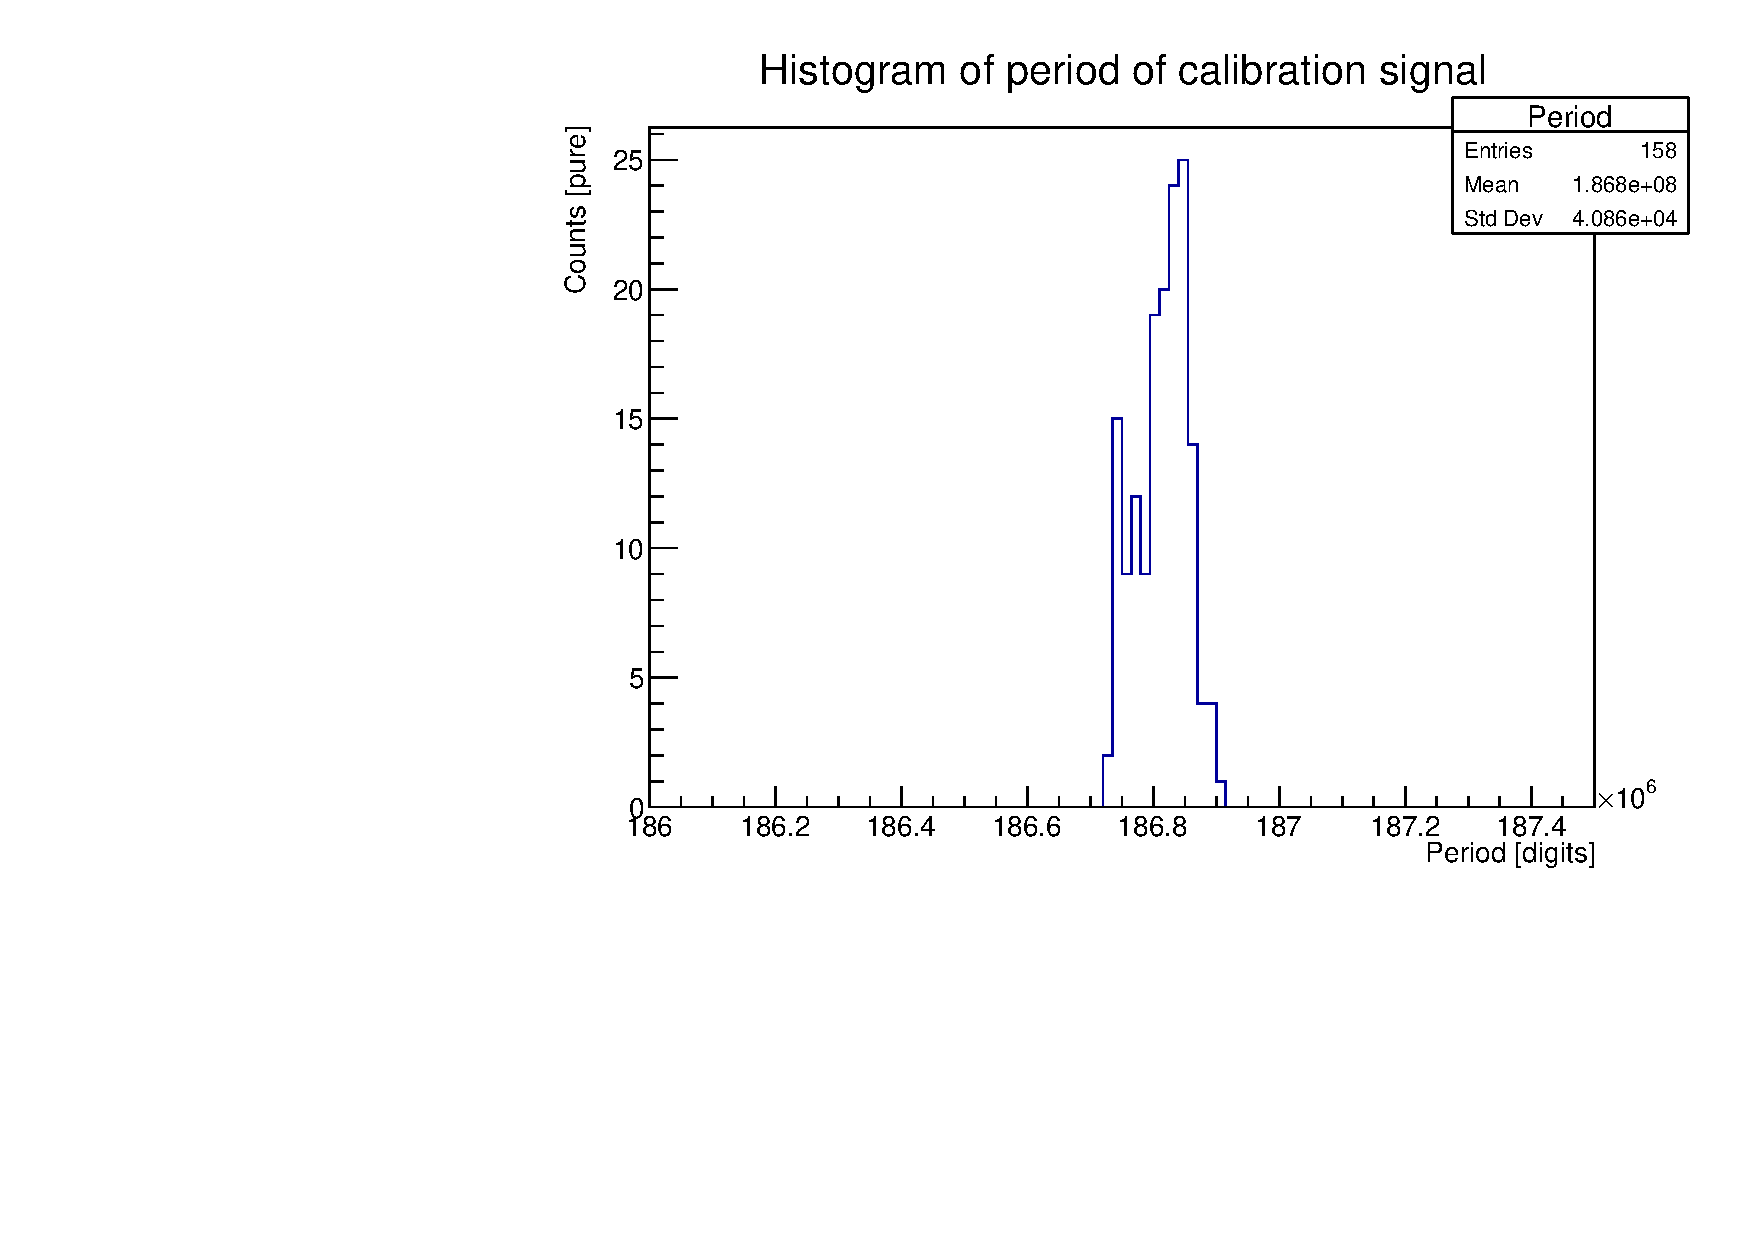
\includegraphics[width=0.7\linewidth]{Periodo.pdf}
    \caption{Istogramma per i periodi del segnale di calibrazione}
    \label{fig:placeholder}
\end{figure}

Quindi, chiamata $\alpha = T[s]/T[dgt]$ la costante di calibrazione digit-tempo $\alpha = 4.98892 \pm 0.00002 $ ns/dgt. 

Per completezza abbiamo misurato anche il ritardo fra due canali (lo 0 e l'1), mandando due onde quadre in fase fra loro per vedere se vi era un ritardo dovuto all'acquisizione.

\begin{figure}[H]
    \centering
    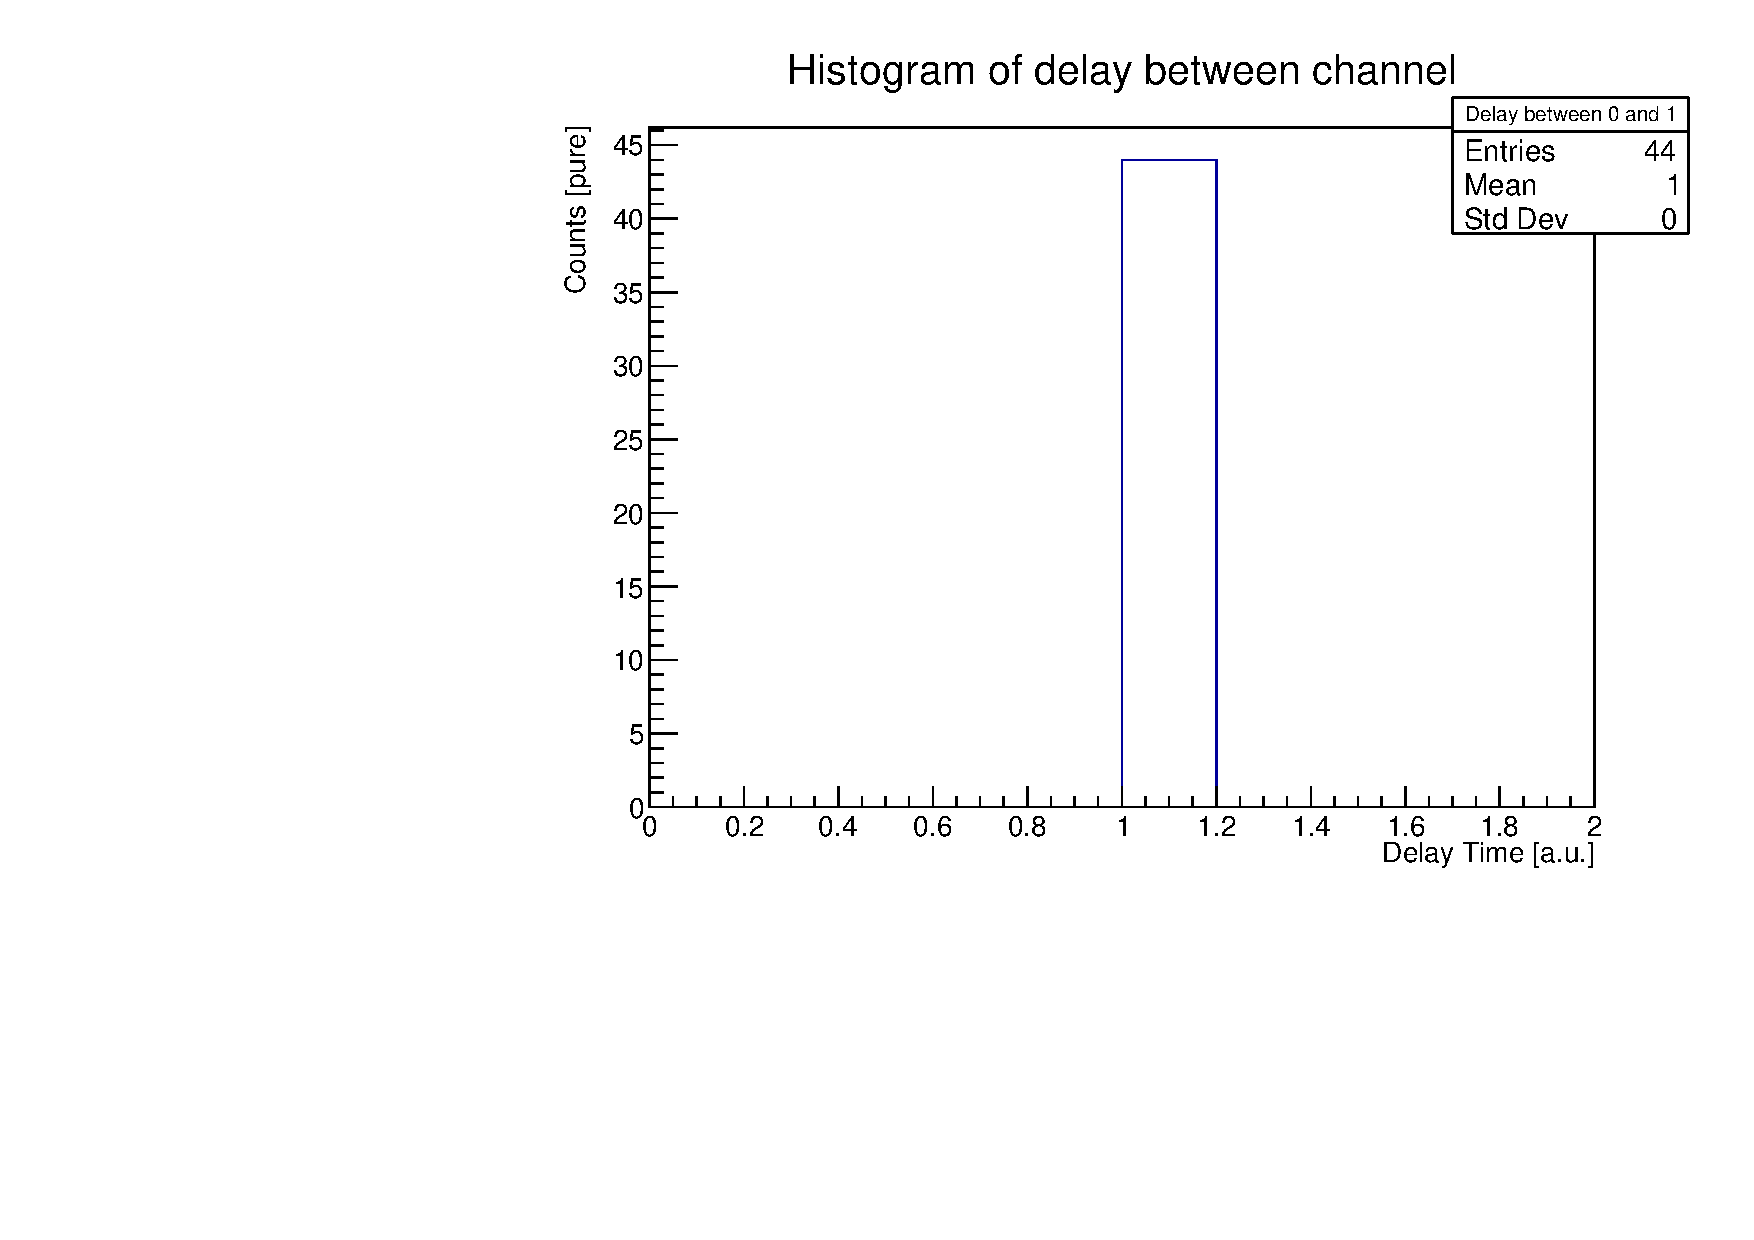
\includegraphics[width=0.7\linewidth]{Ritardo.pdf}
    \caption{Istogramma per i periodi fra i segnali}
    \label{fig:placeholder}
\end{figure}

Il grafico mostra che abbiamo un digit di differenza fra i due canali, corrispondente al valore di $\alpha$ in tempo.

\section{Misura della vita media}

\subsection{Analisi dati}

Abbiamo dunque avviato la presa dati. Alla scheda abbiamo collegato il segnale di START, il segnale di STOP, e 4 segnali aggiuntivi ottenuti dalla coincidenza del GATE con ciascuno dei PMT del blocco in OR con il negato del VETO (è fondamentalmente lo STOP con il segnale di un PMT singolo al posto dell'OR).

Usiamo tali informazioni aggiuntive in sede di analisi dati, al fine di migliorare il riconoscimento dell'evento e rimuovere più eventi di fondo. 

Il nostro algoritmo di analisi dati, funziona nel seguente modo :

\begin{itemize}
\item Individua uno START;
\item Controlla ci sia uno STOP, oppure uno STOP con segnale in uno dei PMT, oppure STOP con segnale in due PMT sovrapposti contemporaneamente;
\item Ripete il controllo cercando i casi precedenti o alternativamente segnale in uno dei PMT;
\item Fa la differenza fra lo START trovato all'inizio e il primo 2.
\end{itemize}

\end{document}